\documentclass[../00_main.tex]{subfiles}

\begin{document}

\section{Educational Internship}

\subsection{NASA ESDS}

\begin{frame}{NASA Earthdata}
    \begin{itemize}
        \item NASA Earth Remote Sensing data is available via the Earth Science 
            Data Systems (ESDS) Program (see 
            \href{https://earthdata.nasa.gov/esds}{here})
        \item covers data acquisition, processing, distribution of NASA 
            mission data
        \item data is free and software is open source \cite{esds-website}
    \end{itemize}
\end{frame}

\begin{frame}{NASA GES DISC}
    \begin{itemize}
        \item NASA Goddard Earth Sciences (GES) Data and Information 
            Services Center (DISC) 
        \item provides data on atmospheric composition, water \& energy cycles, 
            and climate variability \cite{gesdisc-about}
        \item provides over 3.3 Petabytes of data \cite{gesdisc-main} 
    \end{itemize}
\end{frame}

\begin{frame}{MERRA--2 Dataset}
    \begin{itemize}
        \item Modern-Era Retrospective analysis for Research and 
            Applications version 2 
        \item historical climate reanalysis using satellite data
        \item specifically M2I3NPASM, Jan. 1 1980 to Oct. 1 2020
    \end{itemize}
\end{frame}

\begin{frame}{M2I3NPASM}
    \begin{itemize}
        \item covers whole globe, measurements every 3 hours \cite{data-summary}
        \item 14 variables with latitude, longitude, time, pressure level
        \item some variables \cite{data-readme}:
            \begin{itemize}
                \item surface pressure
                \item specific humidity
                \item eastward and northward wind
                \item temperature, etc.
            \end{itemize}
    \end{itemize}
\end{frame}

\begin{frame}{M2I3NPASM Cont.}
    \begin{itemize}
        \item data available on GES DISC website (see 
\href{https://disc.gsfc.nasa.gov/datasets/M2I3NPASM_5.12.4/summary}{here})
        \item option to download only a subset of the data 
        \item can be restricted by time, latitude, longitude, group of variables
        \item full file is 1.1 GB in size \cite{data-readme}, selection is
            smaller
        \item I chose 34\textdegree{}N to 48\textdegree{}N and 65\textdegree{}E 
            to 83\textdegree{}E.
    \end{itemize}
\end{frame}

\begin{frame}{M2I3NPASM Cont.}
    \begin{figure}[H]
        \center
        \fbox{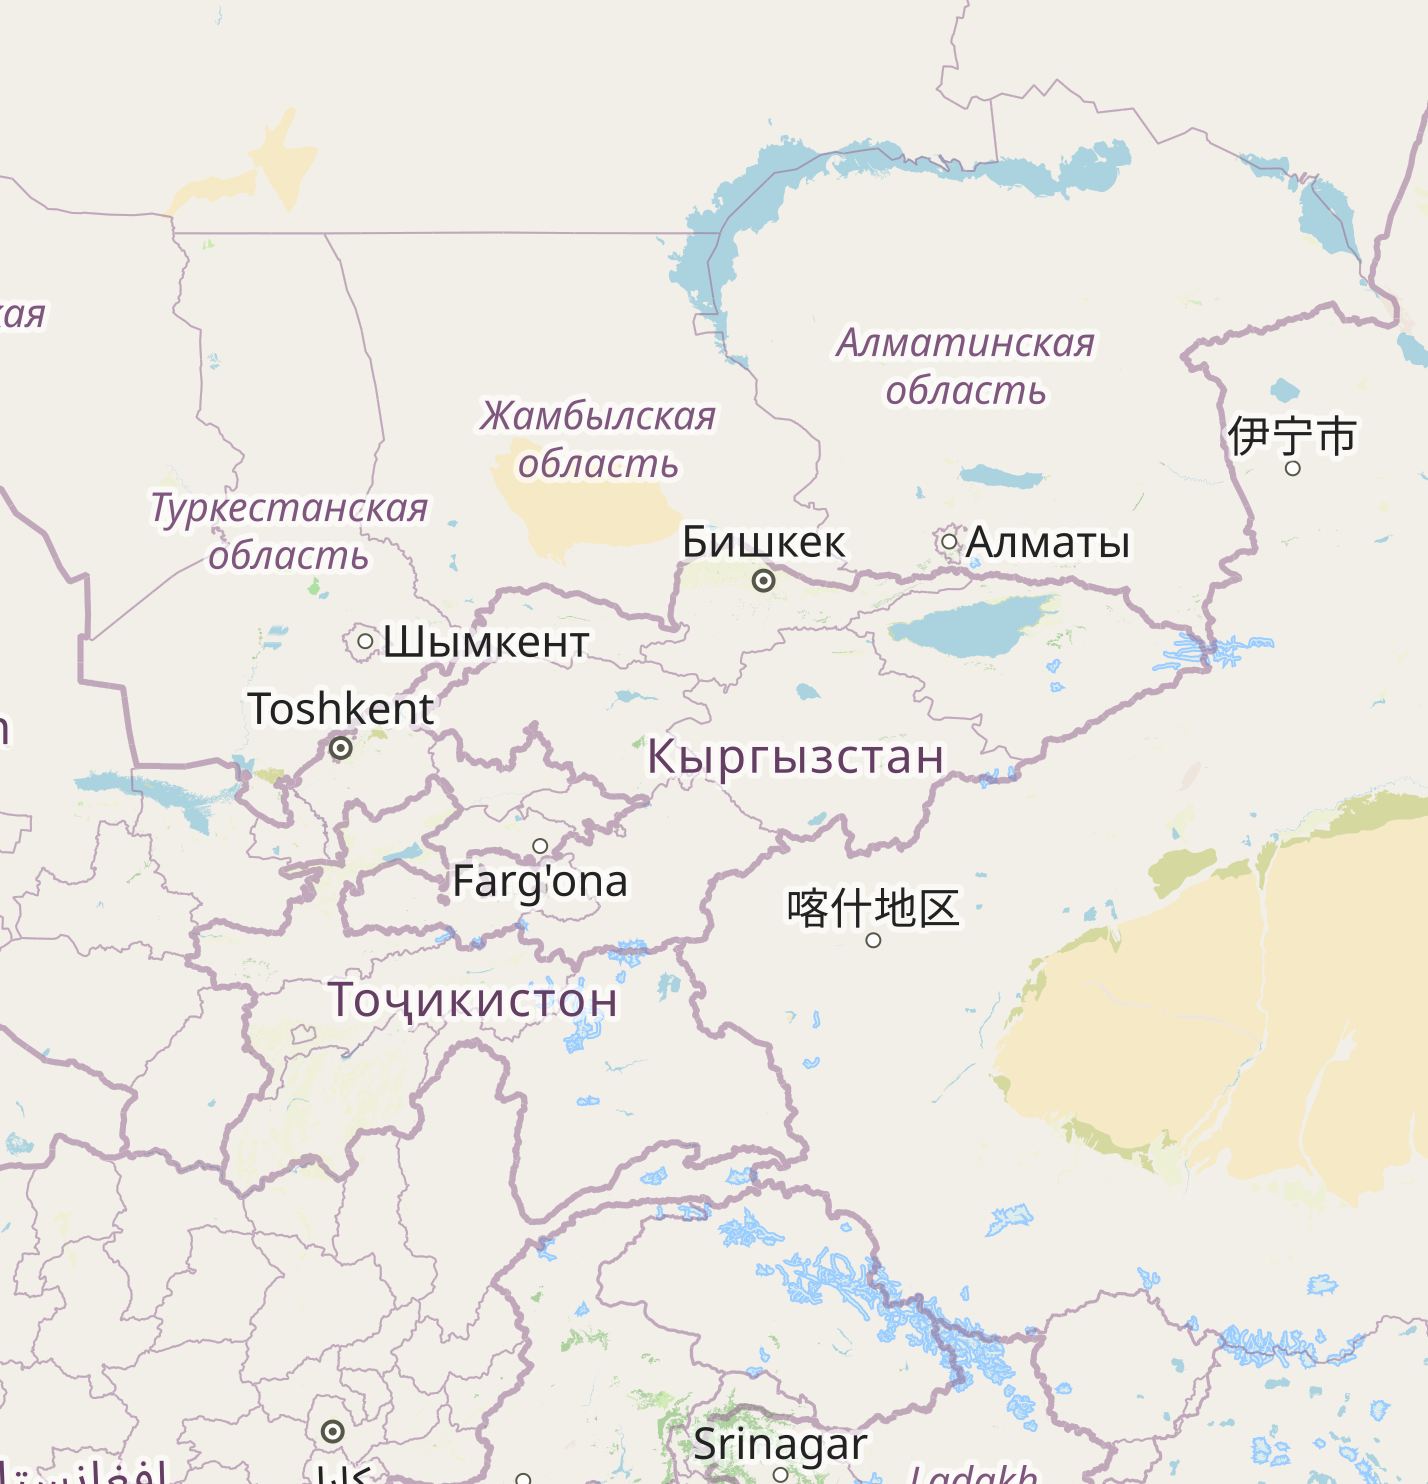
\includegraphics[width=0.7\textheight]{../graphics/map}}
        \caption{OpenStreetMap of the selected region}
        \label{map}
    \end{figure}
\end{frame}

\subsection{NetCDF Format}

\begin{frame}{NetCDF Data Format}
    \begin{itemize}
        \item M2I3NPASM data comes in Network Common Data Form (netCDF)
        \item NetCDF is data format and libraries \cite{netcdf}
        \item developed and maintained by Unidata \cite{unidata}
        \item Unidata maintains libraries for C, Java, Fortran, Python, etc. \cite{netcdf-facts}.
    \end{itemize}
\end{frame}

\begin{frame}{NetCDF and M2I3NPASM}
    \begin{itemize}
        \item netCDF features: self--describing, portable, scalable, 
            appendable, sharable, archivable \cite{netcdf}
        \item M2I3NPASM has 4 dimensions \cite{merra2-files}
            \begin{enumerate}
                \item longitude in degrees east
                \item latitude in degrees north
                \item pressure in hPa
                \item time in minutes since the first time point in a file
            \end{enumerate}
        \item metadata includes fill value, long name, units, etc.
    \end{itemize}
\end{frame}

\subsection{NetCDF Libraries}

\begin{frame}{NetCDF Libraries}
    \begin{itemize}
        \item I am working with Python, thus Python library
        \item NetCDF library for netCDF4 available \cite{netcdf4}
        \item very popular library
        \item I used it to work with the GES DISC data
    \end{itemize}
\end{frame}

\end{document}

\end{document}
